\section{Periodic Orbits}
Using the multi-variable Newton-Raphson scheme described above, periodic solutions can be targeted
in a CR3BP system. In the CR3BP, these periodic solutions exist as members of families that share
similar geometric characteristics. Some of these orbit families are symmetric about a plane or axis
in the rotating frame and this information can be utilized in the targeting process. In addition,
the initial conditions for these families can be obtained through a variety of methods including
linear variational equations about the Lagrange points and bifurcations from other orbit families.

\subsection{Lyapunov Orbit Families}
\subsubsection{A Lyapunov Targeter}
To demonstrate the periodic orbit targeting process, the Newton-Raphson scheme will be used to
solve for a periodic orbit in the $xy$-plane of the rotating frame around the first Lagrange point.
This family of solutions is known as the $L_{1}$ Lyapunov family and they are symmetric about the
$xz$-plane. Therefore, instead of targeting the full orbit, it is only necessary to target half of
it, from one perpendicular crossing of the $xz$-plane to the next. To target one of these orbits at
a specified energy level (Jacobi constant), consider the free variable vector:
\begin{equation}
    \Xbar=\begin{bmatrix}   x_{0}   &   \ydot_{0}   &   \tau    \end{bmatrix}^{T}.
    \label{eq:Lyapunovfreevar}
\end{equation}
Since the boundary value problem being solved starts from a perpendicular crossing, it is only
necessary to allow $x_{0}$ and $\ydot_{0}$ to vary as the rest of the initial states will all be
$0$. In \cref{eq:Lyapunovfreevar}, $\tau$ represents the nondimensional propagation time (TOF) of
the initial conditions. To target another perpendicular crossing for the endpoint of the trajectory
arc, the following constraint vector is used:
\begin{equation}
    \Fbar(\Xbar)=\begin{bmatrix}    y_{f}   &   \xdot_{f}   &   C-C_{d} \end{bmatrix}^{T}=\zerobar,
    \label{eq:Lyapunovconst}
\end{equation}
where $C$ is the Jacobi constant of the propagated arc and $C_{d}$ is the desired Jacobi constant.
The Jacobian matrix is then comprised of partial derivatives from the STM, time derivatives, and
partial derivatives of the Jacobi constant with respect to state variables:
\begin{equation}
    DF(\Xbar)=\begin{bmatrix}   \frac{\partial y_{f}}{\partial x_{0}}                                       &   \frac{\partial y_{f}}{\partial\ydot_{0}}    &   \frac{\partial y_{f}}{\partial\tau}     \\
                                \frac{\partial\xdot_{f}}{\partial x_{0}}                                    &   \frac{\partial\xdot_{f}}{\partial\ydot_{0}} &   \frac{\partial\xdot_{f}}{\partial\tau}  \\
                                \frac{\partial(C-C_{d})}{\partial x_{0}}                                    &   \frac{\partial(C-C_{d})}{\partial\ydot_{0}} &   \frac{\partial(C-C_{d})}{\partial\tau}  \end{bmatrix}
             =\begin{bmatrix}   \phi_{21}                                                                   &   \phi_{25}                                   &   \ydot_{f}                               \\
                                \phi_{41}                                                                   &   \phi_{45}                                   &   \xddot_{f}                              \\
                                2x_{0}-\frac{2(x_{0}+\mu)(1-\mu)}{d^{3}}-\frac{2\mu(x_{0}-1+\mu)}{r^{3}}    &   -2\ydot_{0}                                 &   0                                       \end{bmatrix}.
\end{equation}
This Jacobian matrix can then be used with \cref{eq:NRsolution} to iteratively solve for the free
variable vector $\Xbar$ that solves the provided problem. This provides the initial state and half
of the propagation time for a periodic Lyapunov orbit.

\subsubsection{Lyapunov Initial Guess}
An initial guess for a Lyapunov orbit close to the Lagrange point can come from variational
equations of motion, linearized about the equilibrium point:
\begin{equation}
    x_{0}=x_{L}+\xi,
    \label{eq:xvar}
\end{equation}
\begin{equation}
    \ydot_{0}=-\beta_{3}\xi s,
    \label{eq:ydotvar}
\end{equation}
where $\xi$ is a chosen variation from the $x$-value of the Lagrange point,
\begin{equation}
    \beta_{1}=2-\frac{\frac{\partial U}{\partial x\partial x}+\frac{\partial U}{\partial y\partial y}}{2},
    \label{eq:beta1}
\end{equation}
\begin{equation}
    \beta_{2}=\sqrt{-\frac{\partial U}{\partial x\partial x}\frac{\partial U}{\partial y\partial y}},
    \label{eq:beta2}
\end{equation}
\begin{equation}
    s=\sqrt{\beta_{1}+\sqrt{\beta_{1}^{2}+\beta_{2}^{2}}},
    \label{eq:s}
\end{equation}
\begin{equation}
    \beta_{3}=\frac{s^{2}+\frac{\partial U}{\partial x\partial x}}{2s}.
    \label{eq:beta3}
\end{equation}

The last part of the initial guess for the free variable vector is the half-period of the orbit
$\tau$. This can be approximated by propagating the initial state guess until it reaches the
$x$-axis.

\subsubsection{Converged Lyapunov Orbit}
The linear variational equations are only approximate the dynamics very close to the Lagrange
point. Using $\xi=0.005$ as the initial variation in the $x$-direction from the $L_{1}$ Lagrange
point in the Earth-Moon system:
\begin{equation}
    \Xbar_{0}=\begin{bmatrix}   0.841915    &   -0.0418614  &   1.29755\end{bmatrix}^{T},
    \label{eq:Lyapunovguess}
\end{equation}
and from the guess for the initial state, $C_{d}=3.186877$. This initial free variable guess is
propagated using the CR3BP equations of motion and is represented by the dashed curve in
\cref{fig:Lyapunov}. After targeting a perpendicular crossing using the targeter described above,
the solution can be propagated (for $2\tau$) to obtain the full periodic Lyapunov orbit, shown as
a closed, solid curve in \cref{fig:Lyapunov}. Note that while the energy of the converged solution
matches that of the initial guess, the $x$- and $\ydot$-values have shifted slightly.

\begin{figure}[ht]
    \centering
    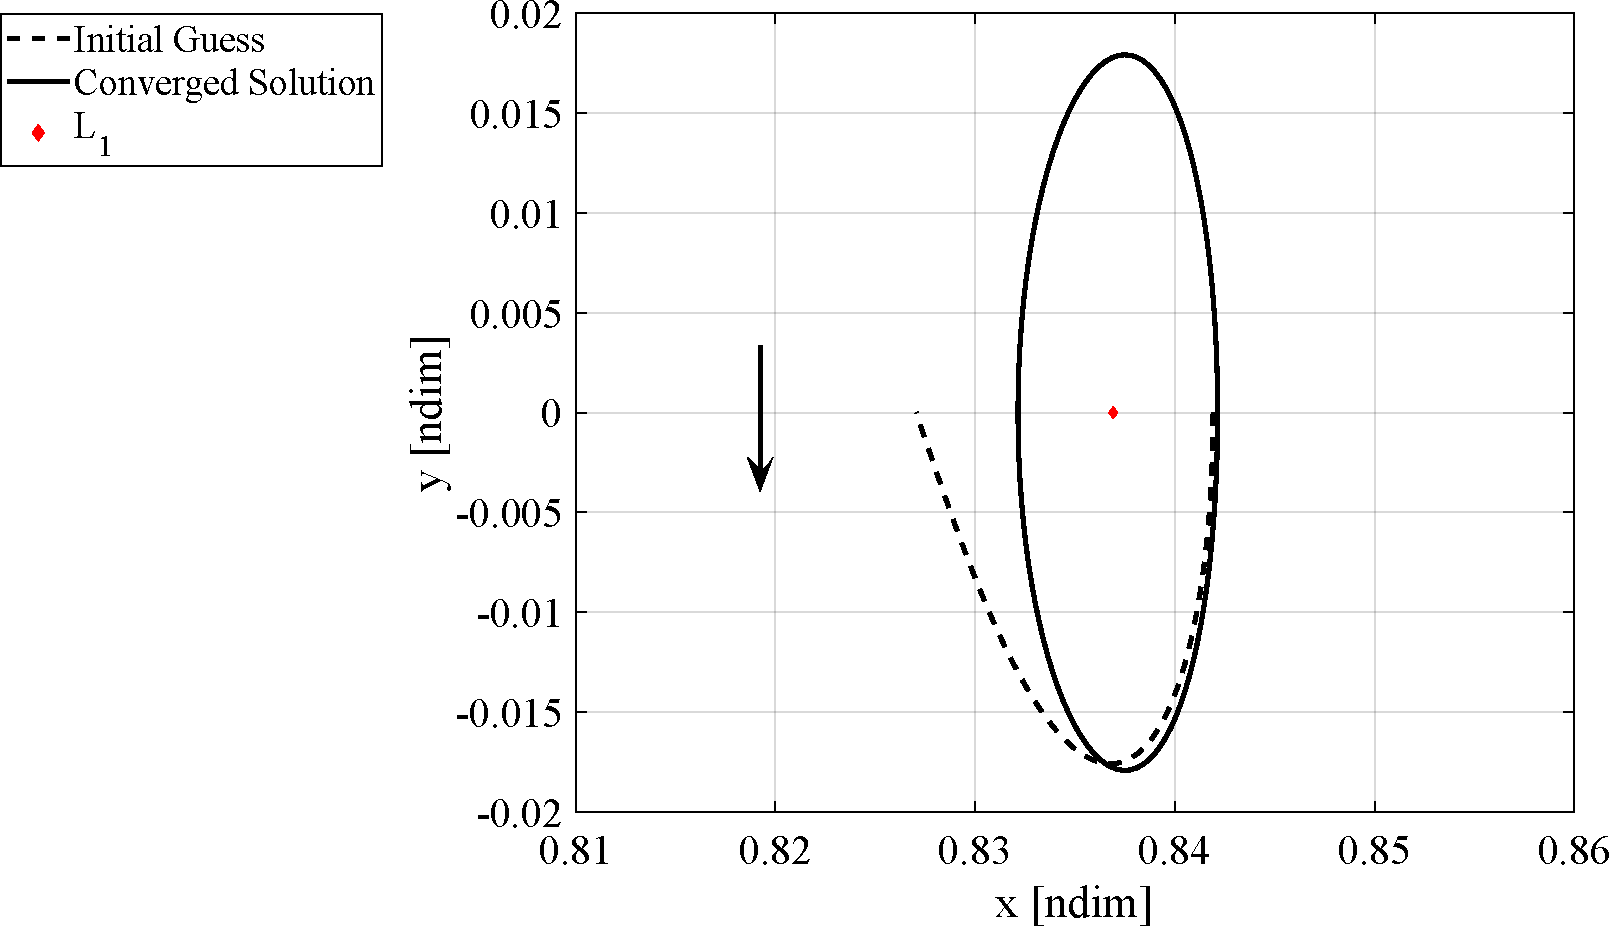
\includegraphics[width=0.75\textwidth]{figures/Lyapunov.pdf}
    \caption{Converged periodic Lyapunov orbit in the Earth-Moon barycentric rotating frame.}
    \label{fig:Lyapunov}
\end{figure}

\subsubsection{Natural Parameter Continuation}
The process described above produces a single solution near the Lagrange point. In order to compute
more solutions (orbits) in the family, especially further away from the Lagrange point where the
linear variational equations no longer apply, converged solutions can be used in a continuation
scheme to find other family members. This investigation utilizes natural parameter continuation,
where one of the parameters of a converged solution is changed by a small amount. This new guess
for an orbit is then converged, and a new solution is obtained. This continuation process can then
be repeated until the scheme reaches a natural/dynamical end or a desired orbit is reached. Natural
parameters of the orbit include (but are not limited to) components of the initial state, the
period, or the Jacobi constant. \cref{fig:L1Lyapunov} shows a large portion of the $L_{1}$ Lyapunov
family in the Earth-Moon system, continued in Jacobi constant from the orbit in
\cref{fig:Lyapunov}. Lyapunov families also exist about $L_{2}$ and $L_{3}$ and can be computed via
the same process. Since $L_{2}$ Lyapunovs are also used in this investigation, they are shown in
\cref{fig:L2Lyapunov}.

\begin{figure}[ht]
    \centering
    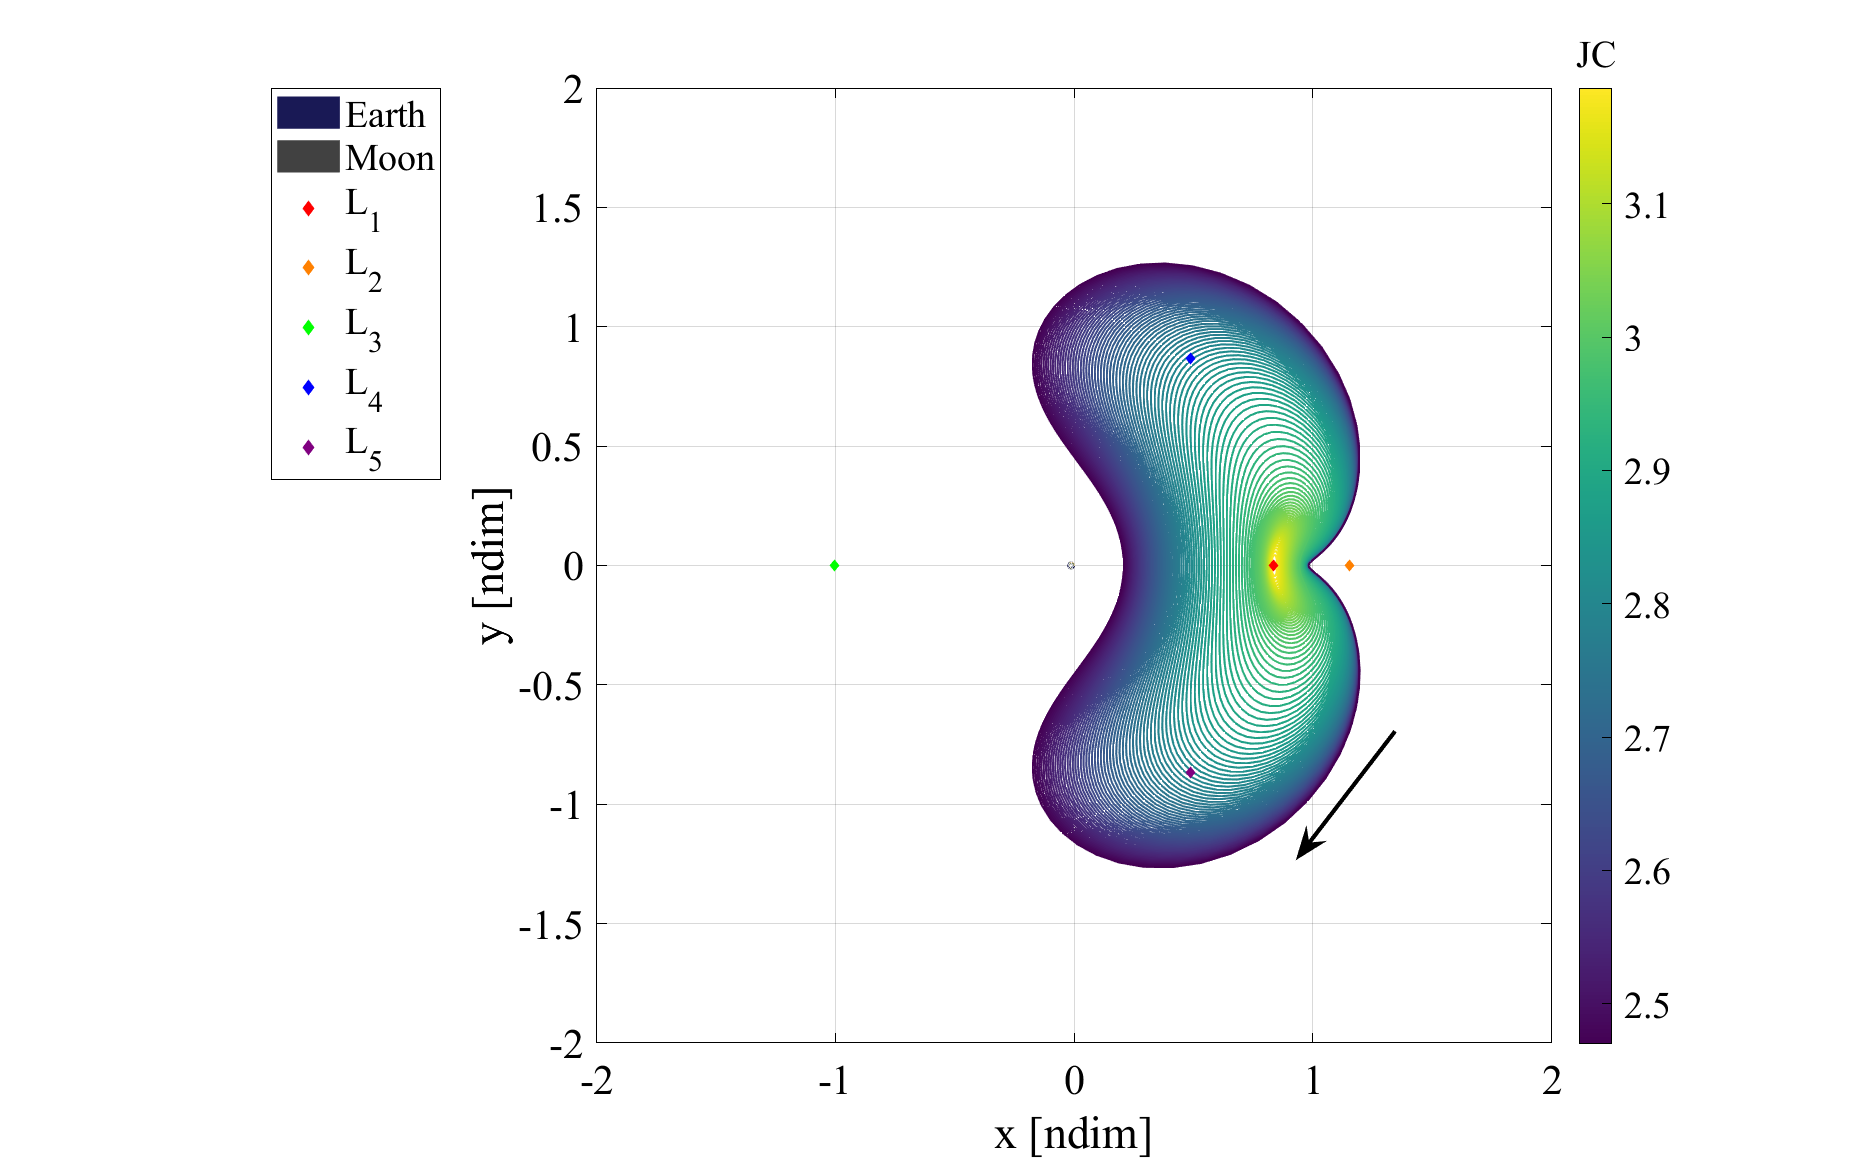
\includegraphics[width=0.9\textwidth]{figures/L1LyapunovFamily.pdf}
    \caption{$L_{1}$ Lyapunov orbit family.}
    \label{fig:L1Lyapunov}
\end{figure}

\begin{figure}[ht]
    \centering
    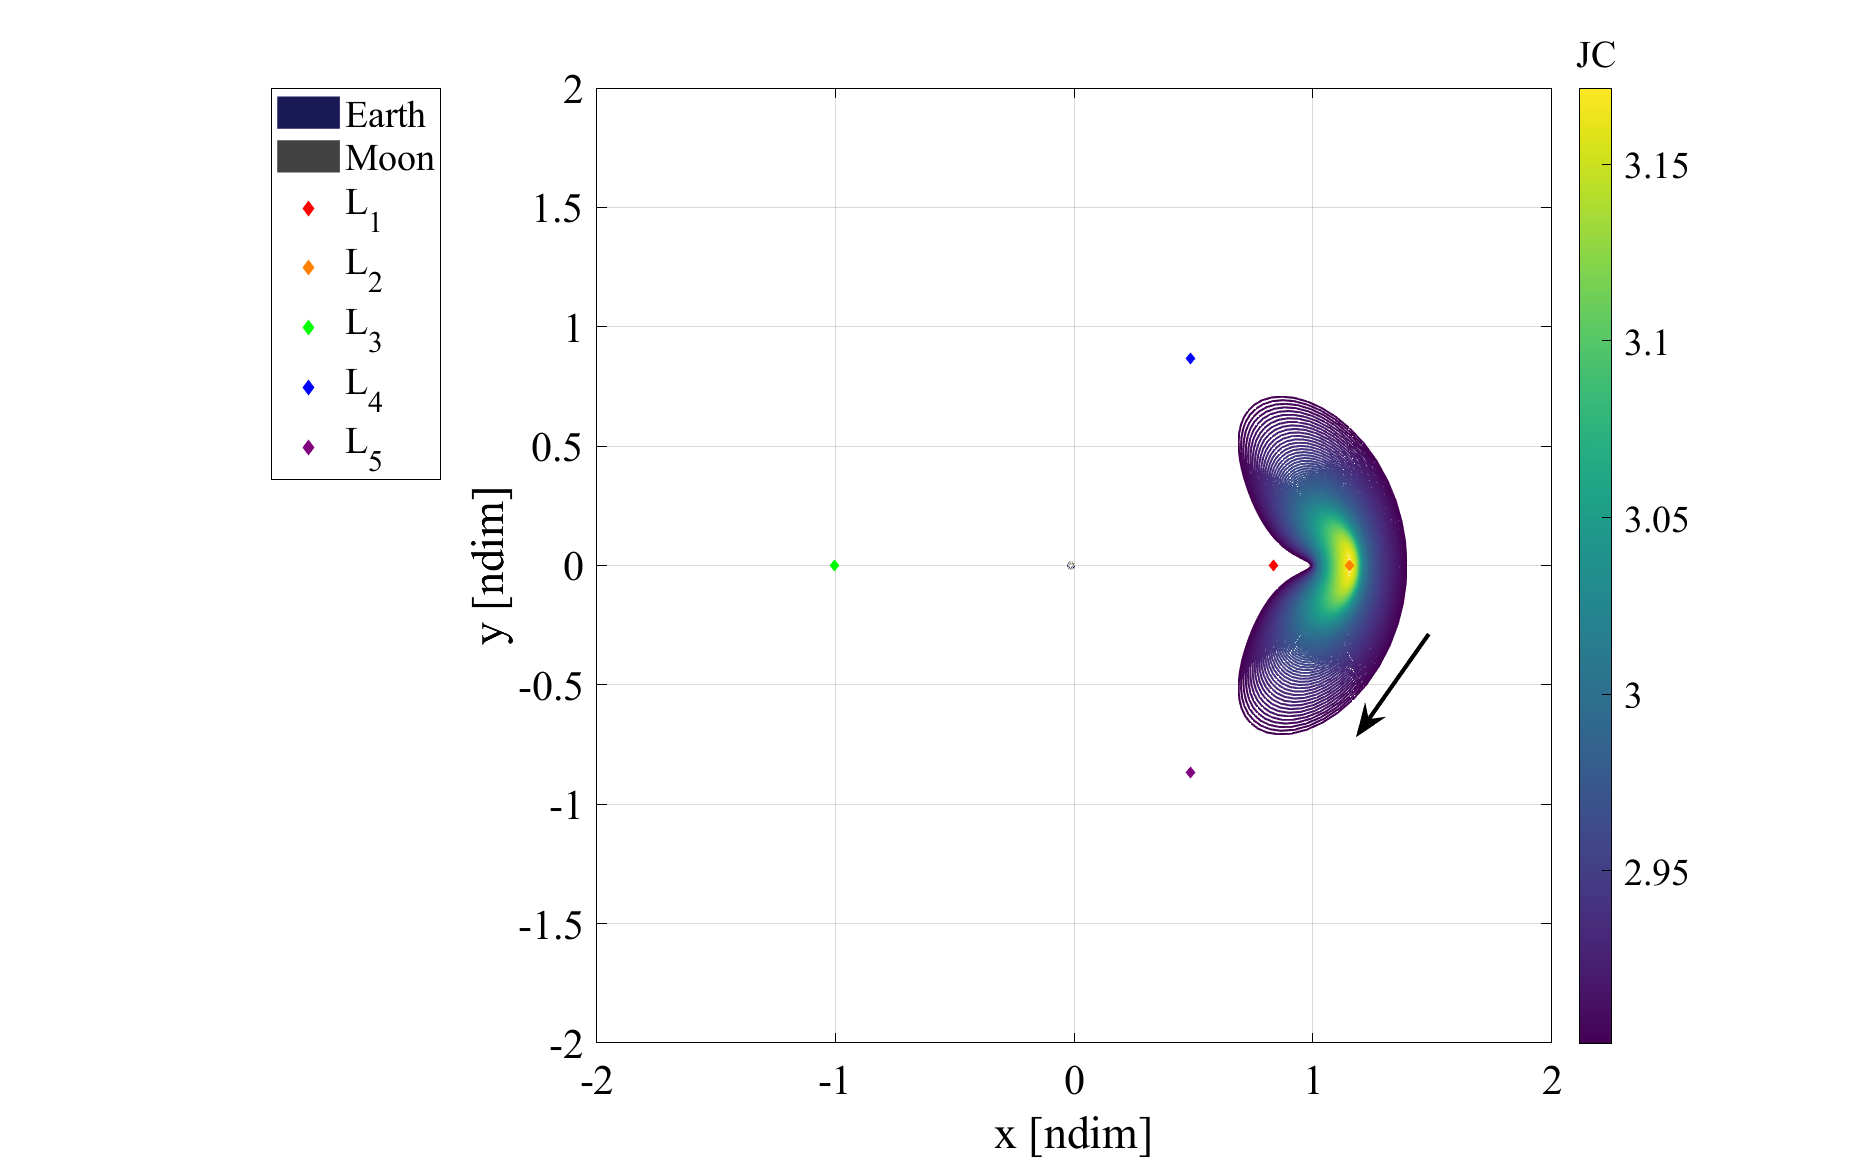
\includegraphics[width=0.9\textwidth]{figures/L2LyapunovFamily.pdf}
    \caption{$L_{2}$ Lyapunov orbit family.}
    \label{fig:L2Lyapunov}
\end{figure}

\subsection{Stability}

